\documentclass[11pt,a4paper,oneside]{book}

% Include the configuration file for layout.
\usepackage{setspace}
\usepackage{geometry}
\usepackage[toc,page]{appendix}
\usepackage{lipsum}
\usepackage[export]{adjustbox}
\usepackage[T1]{fontenc}
\usepackage{textcomp}
\usepackage{epsfig,graphics}
\usepackage{graphicx}
\usepackage{titlesec}


%%%%%%%%%%%%%%%%%%%%%%%%%%%%%%%%%%%%%%%%%%%%%%%%%%%%%%%%%%%%%%%%%%%%%%%%%%%%%%
% Details of your dissertation
%%%%%%%%%%%%%%%%%%%%%%%%%%%%%%%%%%%%%%%%%%%%%%%%%%%%%%%%%%%%%%%%%%%%%%%%%%%%%%

% Insert the correct title etc. into the following commands.
\newcommand{\projectTitle}{<Provisional title of Project>}
\newcommand{\fullname}{<Full Name of Author>}
\newcommand{\degreeTitle}{<Name of Degree Programme>}
	% e.g. BSc Computer Science
\newcommand{\session}{<Session/Academic year>}
	% e.g. 2021/22
\newcommand{\module}{<Module code and name>}
	% e.g. COMP3931 Individual Project

%%%%%%%%%%%%%%%%%%%%%%%%%%%%%%%%%%%%%%%%%%%%%%%%%%%%%%%%%%%%%%%%%%%%%%%%%%%%%%
% Change the geometry of the page to have a 25 mm binding edge
%%%%%%%%%%%%%%%%%%%%%%%%%%%%%%%%%%%%%%%%%%%%%%%%%%%%%%%%%%%%%%%%%%%%%%%%%%%%%%
 \geometry{
 a4paper,
 total={210mm,297mm},
 left=25mm,
 right=25mm,
 top=25mm,
 bottom=20mm,
 }
 
%%%%%%%%%%%%%%%%%%%%%%%%%%%%%%%%%%%%%%%%%%%%%%%%%%%%%%%%%%%%%%%%%%%%%%%%%%%%%%
% Commands to set the line spacing
%%%%%%%%%%%%%%%%%%%%%%%%%%%%%%%%%%%%%%%%%%%%%%%%%%%%%%%%%%%%%%%%%%%%%%%%%%%%%%
 %\singlespacing
 \onehalfspacing
 %\doublespacing
 

%%%%%%%%%%%%%%%%%%%%%%%%%%%%%%%%%%%%%%%%%%%%%%%%%%%%%%%%%%%%%%%%%%%%%%%%%%%%%%
% Some shortcuts that maybe useful
%%%%%%%%%%%%%%%%%%%%%%%%%%%%%%%%%%%%%%%%%%%%%%%%%%%%%%%%%%%%%%%%%%%%%%%%%%%%%%
\DeclareTextCommandDefault{\textcopyright}{\textcircled{c}}
 
%%%%%%%%%%%%%%%%%%%%%%%%%%%%%%%%%%%%%%%%%%%%%%%%%%%%%%%%%%%%%%%%%%%%%%%%%%%%%%
% Bibliography style: choose one and make sure you have the relevant .bst file
%%%%%%%%%%%%%%%%%%%%%%%%%%%%%%%%%%%%%%%%%%%%%%%%%%%%%%%%%%%%%%%%%%%%%%%%%%%%%%
\bibliographystyle{abbrv}


%%%%%%%%%%%%%%%%%%%%%%%%%%%%%%%%%%%%%%%%%%%%%%%%%%%%%%%%%%%%%%%%%%%%%%%%%%%%%%
% Layout for the front cover !!!!! YOU SHOULD NOT HAVE TO CHANGE THIS!!!!!
%%%%%%%%%%%%%%%%%%%%%%%%%%%%%%%%%%%%%%%%%%%%%%%%%%%%%%%%%%%%%%%%%%%%%%%%%%%%%%
 
\newcommand{\frontcover}{
% The title page:
\begin{titlepage}
\newgeometry{left=25mm,right=25mm,top=70mm,bottom=5mm}

\begin{minipage}[t]{6cm}
\noindent\textbf{\Large{School of Computing}}\\
{\fontfamily{ptm}\selectfont 
\uppercase{faculty of engineering and physical sciences}
}
\end{minipage}
\hfill
\begin{minipage}[t]{7cm}
\vspace*{-15pt}

\includegraphics[scale=0.2,right]{logo_black.png}
\vspace*{-1pt}
\end{minipage}

\noindent\makebox[\linewidth]{\rule{\paperwidth}{0.4pt}}

\centering
\vspace*{20mm}
\textbf{\huge Project Outline And Plan}\\
\vspace*{17mm}
\textbf{\Large\projectTitle}\\
\vspace*{10mm}
\textbf{\large\fullname}\\
\vspace*{10mm}
\textbf{\degreeTitle}\\
\vspace*{10mm}
\textbf{\module}\\

\vfill

\noindent The candidate confirms that the work submitted is their own and the appropriate credit has been given where reference has been made to the work of others.
\vspace{5mm}\\
\noindent I understand that failure to attribute material which is obtained from another source may be considered as plagiarism.
\vspace{10mm}\\
\flushright(Name of Student) \fullname
\flushleft
\vfill
\textcopyright~\session~The University of Leeds and~\fullname
\vspace*{10mm}
\restoregeometry
\end{titlepage}
}

\begin{document}
% The prelude is everything up to the start of chapter 1, and is contained
% in a file called "prelude.tex".
\pagenumbering{roman}
\frontcover

\clearpage

\noindent The candidate confirms that the following have been submitted.\\

% Below are examples of what your deliverables may be,
% but since every project is different, not all deliverables
% apply to all projects. Having said that, you should have
% the 'Final Report' deliverable, and most projects will also
% have a link to an online software repository.

\begin{table}[ht!]
\begin{tabular}{|p{0.3\textwidth}|p{0.3\textwidth}|p{0.3\textwidth}|}
\hline 
Items & Format & Recipient(s) and Date \\ 
\hline 
Final Report & Hard copy and PDF file & Hard-copy handed to SSO (DD/MM/YY); PDF uploaded to Minerva (DD/MM/YY) \\ 
\hline 
<Example> Participant consent forms & PDF file / archive & Uploaded to Minerva (DD/MM/YY) \\ 
\hline 
<Example> Link to online code repository & URL & Sent to supervisor and assessor (DD/MM/YY) \\ 
\hline 
<Example> User manuals & PDF and/or hard copy & Sent to client and supervisor (DD/MM/YY) \\ 
\hline 
\end{tabular} 
\end{table}


\vfill

\noindent The candidate confirms that the work submitted is their own and the appropriate credit has been given where reference has been made to the work of others.

\vfill

\noindent I understand that failure to attribute material which is obtained from another source may be considered as plagiarism.

\vfill

% Sign this with a pen for all of the hard copies before you hand
% them over to the SSO. If for any reason the submission of final reports
% is online-only, replace the '\rule{}{}' command with your name.
\flushright(Signature of Student) \rule{50mm}{1pt}
\flushleft

\vfill

\textcopyright~\session~The University of Leeds and~\fullname
% Summary

\begin{dissertationsummary}
<Concise statement of the problem you intended to solve and main achievements (no more than one A4 page)>
\end{dissertationsummary}

\clearpage
\centering\textbf{Acknowledgements}
\flushleft
I would like to thank my supervisor Dr. Samuel Wilson for his guidance and support.


% The contents
\tableofcontents

% The list of figures and tables. Optional.
%\clearpage
%\listoffigures
%\listoftables

\pagenumbering{arabic}


% Include as many chapters as you have.
% The "chapter1.tex" etc. files should be in a directory called "chapters"
\setlength\parindent{20pt}
\chapter{Introduction and Background Research}

% You can cite chapters by using '\ref{chapter1}', where the label must
% match that given in the 'label' command, as on the next line.
\label{chapter1}

% Sections and sub-sections can be declared using \section and \subsection.
% There is also a \subsubsection, but consider carefully if you really need
% so many layers of section structure.
\section{Introduction}
\label{chapter1:introduction}

Operating systems (OSes) are specialised, low level software that manage a computer's
resources and provides a common interface for programs. The most common operating
systems used by most consumers today include MacOS and Windows. Xv6 is an operating
system written by MIT for the purposes of teaching, which runs on the RISC-V architecture \cite{xv6:book}\cite{xv6:code}.
As it is meant to be a teaching OS, it has very barebones functionality,
which includes a command line shell and some basic user programs by default.

This project aims to extend Xv6 with some graphics functionality.


% Must provide evidence of a literature review. Use sections
% and subsections as they make sense for your project.
\section{Background research}
\subsection{Xv6}
As mentioned in Chapter \ref{chapter1:introduction}, Xv6 is a barebones OS used for teaching purposes developed by MIT.
Its features include:
\begin{itemize}
    \item Based on UNIX v6 (hence the v6 in Xv6)
    \item Written for 64 bit RISC-V architecture
    \item Multicore support with a round robin scheduler
    \item Runs on QEMU (qemu-system-riscv64)
\end{itemize}

\subsection{QEMU}
QEMU is an emulator that allows running a guest operating system that may run on
a different target hardware platform. In our case we will be running Xv6,
which runs on the RISC-V architecture, in QEMU for development and testing.


It also provides a way to debug the kernel through a GDB serial port, which greatly
eases development and testing as we can connect a graphical debugger to the kernel.


We will also be using its device emulation to emulate a VGA card on the PCI bus 
for our driver to communicate with to display graphics. It offers many options 
each with its own pros and cons ranging from a simple VGA device with a linear framebuffer
to cards with hardware acceleration. Additionally, QEMU also
provides a simulated display that can be viewed through a VNC client, so we can
see the graphics output of Xv6.

\subsection{VGA}
VGA (Video Graphics Array) has a well defined but complex hardware standard.
Although complex, there is an abundance of technical resources
\cite{vgamanual}
\cite{osdevvga}
\cite{freevga}
that can
assist in developing a VGA driver. In addition, QEMU can emulate a VGA
graphics card.

\subsection{PCI}
PCI (Peripheral Component Interconnect) is a standard that allows the communication of external hardware peripherals. 
This is how we will interface with the emulated VGA card to display graphics.

\subsection{Hardware interfacing with Xv6}
\label{chapter1:research:hardware}
To find the emulated VGA card connected to system, we can walk the PCI
configuration space and search for the Device ID and Vendor ID of the card.
Usually the preferred method would be to walk the device tree \cite{devicetree} to find
the hardware configuration and memory mapped addresses, but since we are running
on the QEMU 'virt' machine we can hardcode these addresses for now.

\begin{listing}[!ht]
\begin{minted}{c}
static const MemMapEntry virt_memmap[] = {
    [VIRT_DEBUG] =       {        0x0,         0x100 },
    [VIRT_MROM] =        {     0x1000,        0xf000 },
    [VIRT_TEST] =        {   0x100000,        0x1000 },
    [VIRT_RTC] =         {   0x101000,        0x1000 },
    [VIRT_CLINT] =       {  0x2000000,       0x10000 },
    [VIRT_ACLINT_SSWI] = {  0x2F00000,        0x4000 },
    [VIRT_PCIE_PIO] =    {  0x3000000,       0x10000 },
    [VIRT_PLIC] =        {  0xc000000, VIRT_PLIC_SIZE(VIRT_CPUS_MAX * 2) },
    [VIRT_UART0] =       { 0x10000000,         0x100 },
    [VIRT_VIRTIO] =      { 0x10001000,        0x1000 },
    [VIRT_FW_CFG] =      { 0x10100000,          0x18 },
    [VIRT_FLASH] =       { 0x20000000,     0x4000000 },
    [VIRT_PCIE_ECAM] =   { 0x30000000,    0x10000000 },
    [VIRT_PCIE_MMIO] =   { 0x40000000,    0x40000000 },
    [VIRT_DRAM] =        { 0x80000000,           0x0 },
};
\end{minted}
\caption{/hw/riscv/virt.c:45-61 from the QEMU source code \cite{qemusource}}
\label{listing:1}
\end{listing}

\begin{figure}[H]
    \centering
    \includegraphics[width=8cm]{Pci-config-space.png}
    \caption{PCI Configuration Space Header Format \cite{figure:pciecamheader}}
    \label{figure:1}
\end{figure}

As shown in listing \ref{listing:1}, the QEMU `virt' machine has defined mappings 
for the PCI configuration space, memory mapped IO and port IO 
(\mintinline{c}{[VIRT_PCIE_ECAM]}, \mintinline{c}{[VIRT_PCIE_MMIO]}, \mintinline{c}{[VIRT_PCIE_PIO]} respectively).
Using this information, and the configuration space layout described by figure \ref{figure:1},
finding the card by walking the configuration space table searching for the corresponding IDs 
should be trivial. Setting up and communicating with the card can be achieved by using
the Base Address Registers in the configuration space to set the MMIO addresses for the framebuffer
and the port IO to configure the card as documented in \cite{osdevvga} can be done through the
memory mapping for \mintinline{c}{[VIRT_PCIE_PIO]}.
% TODO: add reference to BAR!

\subsection{Window managers}
\label{chapter1:research:winman}
A window manager is required for multiple user space programs to share the screen. Otherwise
concurrent graphical user programs would try to write to the same display and overwrite each other.

\subsubsection{Windows}
Windows provides a windowing system that provides free floating windows that can be created
and managed using the Windows API \cite{windowsapi:window}. It is unclear how much of the display
server and compositor is running in user mode or kernel mode.
\subsubsection{Linux - X Windowing System}
The X windowing system also provides free floating windows that is managed by the X Display Server. 
The most commonly used implementation is the open source X.Org project \cite{Xorg}. It is a userspace and unprivileged
display server that communicates with the kernel through display drivers.
\subsubsection{Our implementation}
We'll be taking inspiration from both implementations of windowing systems. For simplicity,
since Xv6 does not have any mouse implementations, a grid window system is a good alternative
that can use hotkeys for window switching. The window manager will sit in the kernel providing 
very basic functionality such as window allocation, input event queuing, and copying
user data on the framebuffer (with bounds checking). This will reduce the attack surface
on the kernel by having the rendering done in unprivileged user mode.

Additionally, we will be exposing the windows as device files, following the Unix mantra
``everything is a file''. This has the advantage of being able to use the included
read and write system calls for communicating with the kernel window manager.

\subsection{Development tools}
\subsubsection{Compile toolchain}
Ubuntu has the tools required for Xv6 compilation in its `apt' software repository. 
To ensure a consistent development environment, Docker will be used to create a 
development container with all the required tools (see Appendix \ref{appendix:c:1})
\subsubsection{Debugging with GDB}
As QEMU provides a serial GDB port to debug the kernel, we will be using GDB to attach to QEMU
to inspect the kernel. GDB can be used to read the debugging symbols, which greatly eases debugging
by allowing us to step through the kernel line by line and set breakpoints at desired lines.
GDB can show the contents of variables during program execution with their original
names. QEMU also supports interrupting the kernel via GDB to stop at its current instruction
and enter step-through debugging, which will be an invaluable tool for infinite loops or deadlocks
in the kernel. 
\subsubsection{IDE}
Visual Studio Code \cite{vscode} is a text editor that supports extensions which can have IDE features,
making it suitable for many use cases. For our use case, it has support for Docker containers and
a GUI for GDB (figure \ref{figure:2}). With its `tasks' functionality as well, VSCode can
be configured to build xv6, run qemu and attach gdb in one shortcut, which will greatly
streamline development.

\begin{figure}[H]
    \centering
    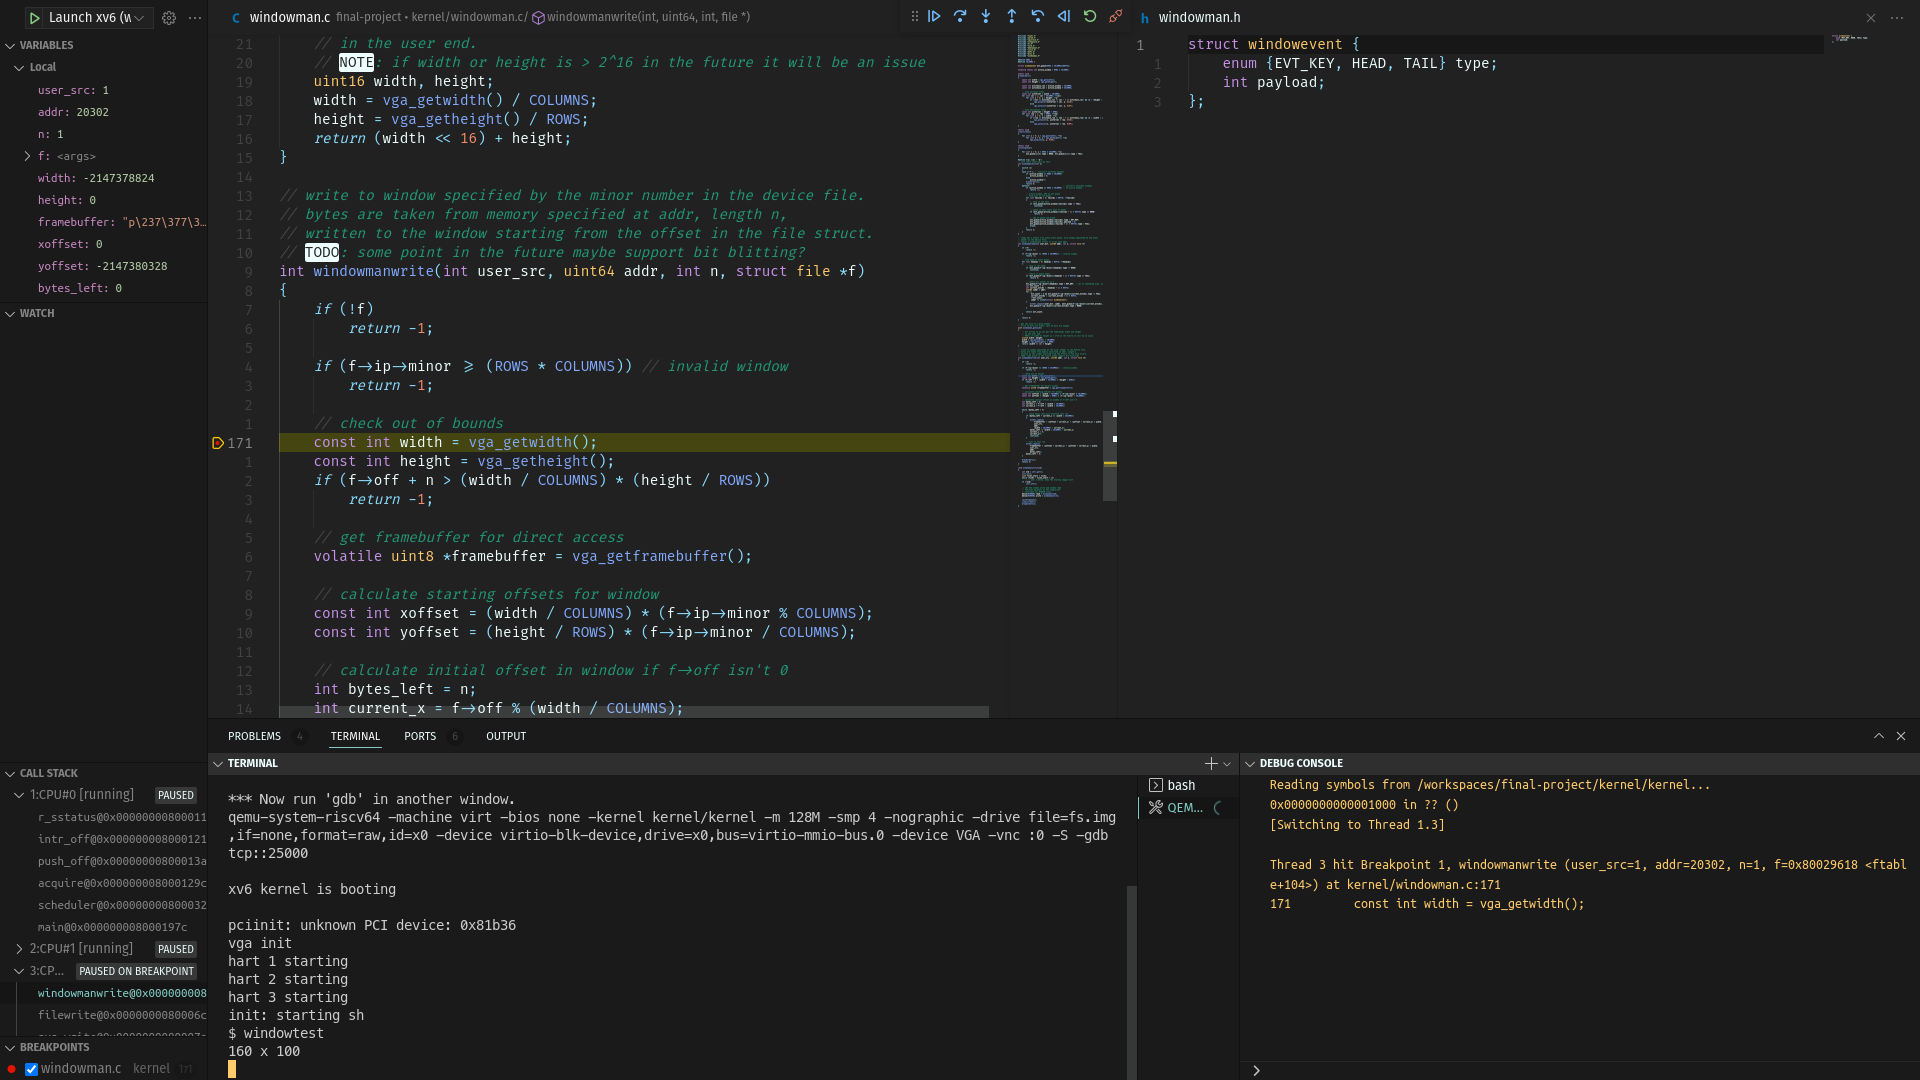
\includegraphics[width=15cm]{Screenshot from 2022-04-26 13-05-47.png}
    \caption{Visual Studio Code Debugging}
    \label{figure:2}
\end{figure}


\chapter{Methods}
\label{chapter2}

\section{Development plan}
\subsection{Model}
The waterfall model will be used following the linear nature of the project. 
Features in the planned software are linearly dependent, and following this model
will allow consistent progress to reach the planned objectives and deliverables.

\subsection{Version control}
As Xv6 is already in a git repository hosted on GitHub \cite{xv6:code}, 
we can simply fork the repository for our modifications. Using git will allow
the progress of the software implementation to be easily documented.

\section{Analysis and design}

\subsection{Running Xv6}
There are two options of running Xv6. This subsection will explore the pros
and cons of both options in this project's use case.
The usual choice is to use QEMU, an emulator that can run systems built for the RISC-V architecture. 

\subsubsection*{Pros}
\begin{itemize}
    \item Xv6 built with QEMU in mind
    \item Extensive debugging capabilities
    \item Easy graphics card and display emulation
    \item Easy to install from the Ubuntu software repositories
\end{itemize}
\subsubsection*{Cons}
\begin{itemize}
    \item Not very performant
\end{itemize}

The alternative option is to run it on bare metal. As there aren't many 
RISC-V processors, the options are limited, with one of the only options being
the `HiFive Unmatched' board by SiFive \cite{hifiveunmatched}.

\subsubsection*{Pros}
\begin{itemize}
    \item Dedicated RISC-V processor, very performant
    \item Ability to observe the solution on real hardware
\end{itemize}
\subsubsection*{Cons}
\begin{itemize}
    \item Expensive, costs USD 665
    \item Would require additional hardware for this project, adding to the already expensive cost of the board
    \begin{itemize}
        \item VGA compatible graphics card
        \item JTAG interface hardware for debugging
    \end{itemize}
    \item Modifications in Xv6 required as some memory addresses are hardcoded for the emulated QEMU `virt' board
\end{itemize}


Given all this, running Xv6 in QEMU is the best option as it will suffice for 
development and testing of a graphics implementation.

\subsection{QEMU VGA emulation}
There are many emulation options for graphics provided by QEMU \cite{qemucards}. 
We will choose the most basic VGA card that we can access through PCI communication.
This card provides full VGA compatibility which can be configured through its data
ports (using the memory mapped PCI port IO addresses), and a linear framebuffer exposed
as memory mapped IO which can be mapped anywhere in the PCI MMIO region of the virtual
address space.

\subsection{Solution diagram}
\begin{figure}[H]
    \centering
    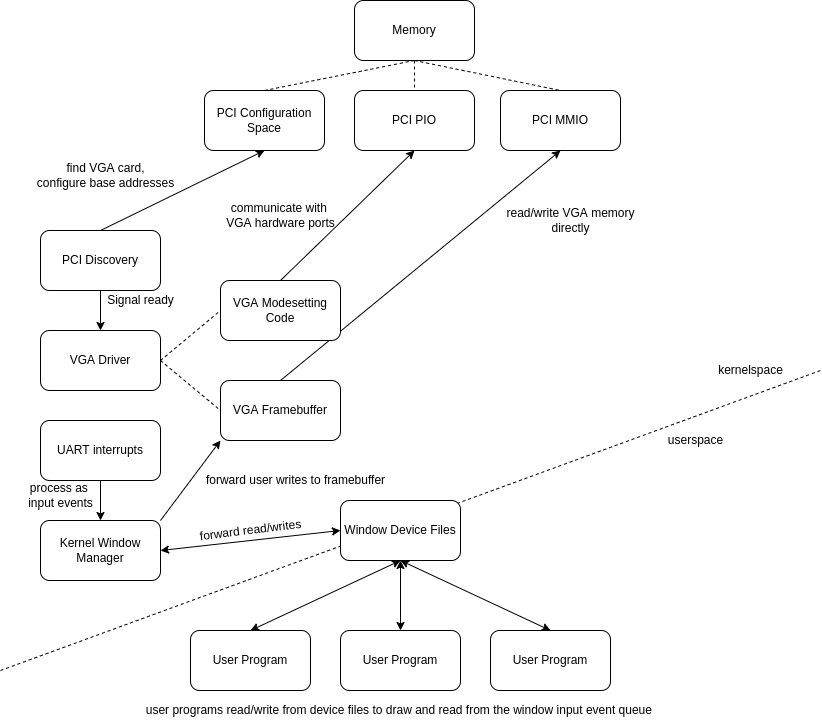
\includegraphics[width=16cm]{diagram.drawio.png}
    \caption{Solution design diagram}
    \label{figure:3}
\end{figure}

The design diagram in figure \ref{figure:3} illustrates how the different parts
of the solution will communicate and interact with each other. In short, the PCI
discovery code will find the VGA card and configure the base addresses, then signal
the driver when the VGA device is ready. 

The VGA driver will provide an interface to the framebuffer and some modesetting code, through the port IO and memory IO which
have address mappings in the virtual address space. The window manager will then use
the framebuffer exposed by the driver to process user code that draws to the screen,
and register UART interrupts as input events to be passed back to user code.

\section{Implementation}

\subsection{Xv6 build modifications}
A Makefile is provided with the Xv6 project that contains tasks that builds the
kernel, user programs, and the filesystem. It also has tasks that runs the compiled
kernel and filesystem image on QEMU.

\subsubsection{QEMU options}
There is a variable called \mintinline{c}{QEMUOPTS} in the Makefile that contains
command line options forwarded to QEMU. We need to add the following line
\begin{minted}{Makefile}
    QEMUOPTS += -device VGA -vnc :0
\end{minted}
to enable the VGA device emulation and serve the display output via VNC. We will also
modify the C compiler flags to include \mintinline{bash}{-O0} to disable all optimisations
during development which could otherwise interfere with debugging.

When creating new files to be compiled into the kernel 
(Chapters \ref{chapter2:impl:pci},\ref{chapter2:impl:driver},\ref{chapter2:impl:winman}),
the appropriate compile targets must be appended to the \mintinline{c}{OBJS} variable. Similarly
for user programs, shared code must be appended to \mintinline{c}{ULIB}, and the programs appended
to \mintinline{c}{UPROGS}.

\subsection{Xv6 memory mapping}
\label{chapter2:impl:memory}
As mentioned earlier in Chapter \ref{chapter1:research:hardware}, the memory addresses for
PCI communication will need to be configured in Xv6. Using the mappings found in the
QEMU source tree in Listing \ref{listing:1}, we can add the following lines into the kernel
pagetable in kernel/vm.c (see Appendix \ref{appendix:c:2} for address definitions).
\begin{minted}[breaklines]{c}
  // map PCI ECAM space
  kvmmap(kpgtbl, PCI_ECAM_BASE, PCI_ECAM_BASE, PCI_ECAM_LEN, PTE_R | PTE_W);

  // map PCI PIO
  kvmmap(kpgtbl, PCI_PIO_BASE, PCI_PIO_BASE, PCI_PIO_LEN, PTE_R | PTE_W);

  // map VGA framebuffer (PCI MMIO)
  kvmmap(kpgtbl, VGA_FRAMEBUFFER_BASE, VGA_FRAMEBUFFER_BASE, VGA_FRAMEBUFFER_SIZE, PTE_R | PTE_W);
\end{minted}
These will configure direct mappings for these addresses for kernel read and write access only, denying execution
or unprivileged access. The kernel is now ready to communicate with the emulated PCI VGA device.
\subsection{PCI communication}
\label{chapter2:impl:pci}
\subsubsection{VGA device discovery}
As shown in figure \ref{figure:1}, the PCI configuration space is a table of PCI configuration headers
where the first 32 bits contain the vendor and device IDs. As documented in the QEMU source tree under
/docs/specs/standard-vga.txt \cite{qemusource}, the ID for the emulated VGA card is 0x11111234.

A simple bruteforce scan through the configuration space, through all 256 PCI buses with 32 devices
per bus, we can compare the first 32 bits of the header with 0x11111234 (see Appendix \ref{appendix:c:3}).

\subsubsection{VGA configuration}
Once the device has been found, we need to write data into the configuration header to achieve the following:
\begin{itemize}
    \item Enable device to respond to port I/O space access, to configure VGA modes and functionality
    \item Enable device to respond to memory space access, for framebuffer access
    \item Configure base address in PCI MMIO address space to expose the framebuffer
\end{itemize}
This can be achieved by the following code snippet, given that `header' is an unsigned 32 bit
pointer to memory.
\begin{minted}{c}
  //-- set bits in the command register
  // Bit 0 - respond to I/O accesses
  // Bit 1 - respond the memory accesses
  // Bit 2 - enable bus mastering (allow card to access other components without CPU intervention)
  header[1] = 0b111;

  __sync_synchronize(); // ensure order of writes aren't modified by optimisation

  // map the framebuffer in our specified base addr
  header[4] = VGA_FRAMEBUFFER_BASE;
\end{minted}

\subsection{VGA graphics driver}
\label{chapter2:impl:driver}
\subsubsection{VGA register access through PCI PIO}
VGA hardware is configured through many 8 bit registers, but the hardware only occupies
a very short port I/O range \cite{osdevvga}. Access is done through indexing, where a register
index is written to a port, then data is written/read for the same or adjacent port. On cases
where data is fed into the same port as the index, an access operation on a specified ``mode setting'' port
will set the port into index mode.

We can see this functionality in the code snippet in listing \ref{listing:2}. The function
handles writing to the VGA registers using ports and register indexes, handling the special cases
mentioned earlier. The read function is also identical, but instead of writing to 
`vga\_pio', the contents of the register index at the given data port offset is returned. Note
that the order of reads and writes are very important here, so we use \mintinline{c}{__sync_synchrnize()}
to emit a memory fence instruction so the compiler and the CPU do not attempt to change the order
of accesses. The \mintinline{c}{__attibute__((unused))} modifier also informs the compiler that
it should not optimise away that variable even though it seems unused, as we need it to perform
a read operation on port 0x3DA to set port 0x3C0 into index mode.

\begin{listing}[H]
    \begin{minted}{c}
static volatile uint8 idx_mode_set __attribute__((unused));
static volatile uint8 *vga_pio = (uint8 *)PCI_PIO_BASE;
static void pwrite(uint32 port, uint32 idx, uint8 val)
{
  if (idx == 0xFF)
  {
    // special case, this port doesn't use indices
    // direct write
    vga_pio[port] = val;
    return;
  }

  // perform a read op on 0x3DA to set 0x3C0 into index mode
  idx_mode_set = vga_pio[0x3DA];
  __sync_synchronize();

  // write the index to the port, and the value to port + 1 if not special case 0x3C0
  vga_pio[port] = idx;
  __sync_synchronize();
  uint write_offset = (port == 0x3C0) ? (uint32)0 : (uint32)1;
  vga_pio[port + write_offset] = val;
  __sync_synchronize();

  // perform a read op on 0x3DA to set 0x3C0 into index mode after
  idx_mode_set = vga_pio[0x3DA];
}
    \end{minted}
    \caption{kernel/pci.c, VGA port write code}
    \label{listing:2}
\end{listing}
\subsubsection{Modesetting}
VGA hardware modes are configured by setting various registers, to configure the timing and resolution
of the output, as well as the colour depth and structure (planar or linear) of the framebuffer.
In non text modes, a palette will also need to be configured for the target colour depth.

For the scope of this project, support for only one mode will be implemented, 320x200 linear 256 colour 
(see Appendix \ref{appendix:c:4} for modesetting value examples).
This mode configures the framebuffer for linear access, with 8 bit (256) colours. This will
also make one pixel equal to one byte, simplifying framebuffer manipulation further in addition to linear access.

Setting the mode can be done by writing the appropriate values to the ports (see kernel/vga.h in the project codebase)
using the port writing logic written in listing \ref{listing:2}.

We will be using the standard VGA 256 colour palette (figure \ref{figure:vgacolor}) for
our implementation. The VGA DAC has a colour subsystem that uses an 18 bit colour
space, 6 bits for each RGB component. We can store this data as a constant in a 32 bit
type array, storing each component in 8 bits (one byte), using only the first 6 bits in each byte.
Writing to the DAC is done in sets of 3, where each component is fed into the DAC data register
sequentially (see listing \ref{listing:palette}).

\begin{figure}
    \centering
    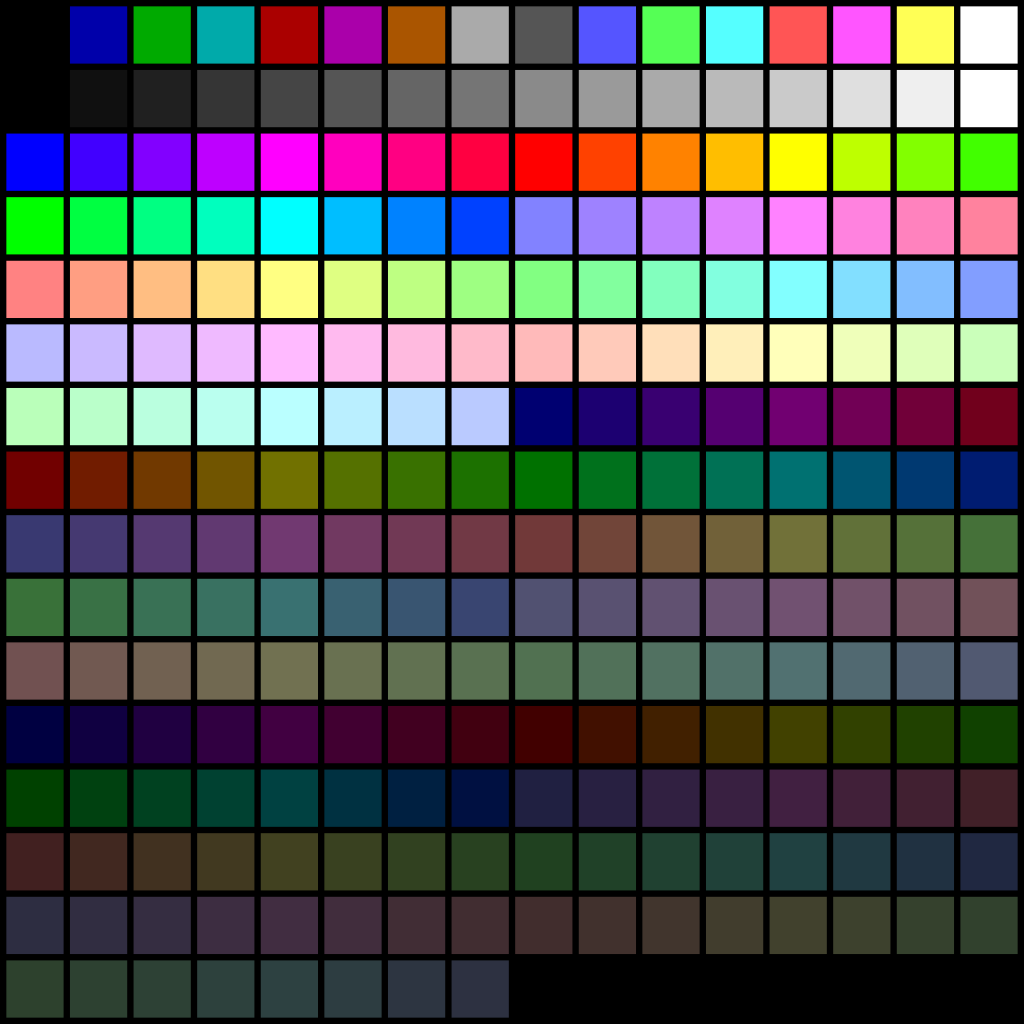
\includegraphics[width=8cm]{1024px-VGA_palette_with_black_borders.png}
    \caption{VGA 256 colour palette}
    \label{figure:vgacolor}
\end{figure}
\begin{listing}
    \begin{minted}{c}
    pwrite(0x3c8, 0xff, 0x00); // set DAC colour register mode to write
    for (int i = 0; i < 256; i++)
    {
      // take 6 bits from relevant part of palette, shift to uint8 type, and write to reg
      // it is 6 bits because the DAC uses an 18 bit colour space, 6 bits per colour component
      pwrite(0x3c9, 0xff, (VGA_256COL_PALETTE[i] & 0xfc0000) >> 18); // set red val
      pwrite(0x3c9, 0xff, (VGA_256COL_PALETTE[i] & 0x00fc00) >> 10); // set green val
      pwrite(0x3c9, 0xff, (VGA_256COL_PALETTE[i] & 0x0000fc) >> 2);  // set blue val
    }
    \end{minted}
    \caption{kernel/vga.c, setting the VGA palette (see listing \ref{listing:2} for pwrite implementation)}
    \label{listing:palette}
\end{listing}

\subsubsection{Boot image}
During system boot, many operating systems display a boot image while it finishes its
boot sequence. Taking inspiration from Linux, the driver will display a boot image, repeated
for every CPU in the system. As each CPU core knows its own CPU number, 
calculating this is trivial, since the width of the screen
and the boot image is known (see Appendix \ref{appendix:c:5}).

\subsection{Grid window manager}
\label{chapter2:impl:winman}

\subsubsection{Device file handling}
As briefly mentioned in Chapter \ref{chapter1:research:winman}, we will be using device files
for programs in userspace to communicate with the window manager. Modifications will need to be
made to file IO handling to register our new device file type (major number) and its handlers
for read/write operations.

Device files are special files that have a major and minor number. For our case,
the major number will indicate that its a `WINDOW' device file with major number 2, with 
the minor number specifying which window the file is referring to. There already
exists another type of device file `CONSOLE' in xv6 with major number 1; this file serves as an
abstraction to reading and writing from the UART console. Similarly for the
window manager, the new device file will be an abstraction for drawing to a window
and reading the window's input events. Using this design pattern saves us from having
to add more system calls to xv6 as well.

\begin{figure}
    \centering
    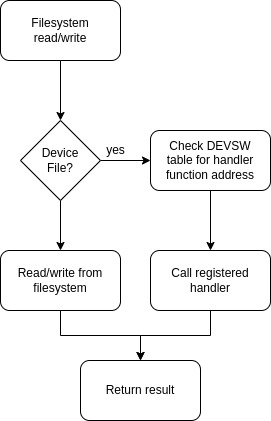
\includegraphics[width=5cm]{fio.drawio.png}
    \caption{Filesystem reads/writes to device files}
\end{figure}

Registering the function handlers to `devsw' is very simple, the addresses for
the read and write handlers are set on
\mintinline{c}{devsw[MAJOR].read} and 
\mintinline{c}{devsw[MAJOR].write} respectively.

Xv6 currently does not pass on the \mintinline{c}{struct file*} pointer.
The function handler signature is \mintinline{c}{(int, uint64, int)}, but we need
details such as the minor number to describe which window and 
the file offset to determine where in the window we start copying data to. We can
simply add the argument for the pointer and modify all the function handlers to 
also expect that argument.

As each window should only be allocated to one program at a time, we can check the
reference count to a device file as it is being opened, and deny access if it already
has an existing reference (another program is using the window).
Since the grid layout also cannot be changed at runtime in the current implementation,
returning the size of the window, the size of the `file' can also be set during opening.
(see listing \ref{listing:winopen})

Note that the function \mintinline{c}{windowman_getsize()} applies some bit tricks
to fit the width and the height into the uint64 type of the file's size. This is done
as the user might find it useful to know the dimensions rather than just the
number of pixels in the window.

\begin{listing}
    \begin{minted}{c}
  if (ip->type == T_DEVICE && ip->major == WINDOW) {
    if (ip->ref > 1) { // only one access per window
      iunlockput(ip);
      end_op();
      return -1;
    }

    ip->size = windowman_getsize();
  }
    \end{minted}
    \caption{Additional checks when opening a window device file}
    \label{listing:winopen}
\end{listing}

\subsubsection{Hooking UART interrupts}
Xv6's only source of input is currently UART. Usually human interaction with
a system is done through keyboard and mouse input, but Xv6 does not support that
and it would be out of scope to implement drivers for those devices. QEMU already
forwards keyboard inputs from the host system as UART inputs, so we will be using
UART as our input.

Currently the console also uses UART for its input as well, as characters are
forwarded to `consoleintr' as they are received in UART (see listing \ref{listing:uartchain}).
We can simply add our window manager handler `windowmanintr' to the chain to also
listen to this input. Note that sometimes we want to `consume' the character 
(not forward it to other listeners), i.e when a window is active the console
should not also receive the input. To achieve this we insert our handler before
the console handler, and check its return value to see if it should call the next
handler in the chain.

\begin{listing}
    \begin{minted}{c}
void
uartintr(void)
{
  // read and process incoming characters.
  while(1){
    int c = uartgetc();
    if(c == -1)
      break;
    if (windowmanintr(c) != 0)
      consoleintr(c);
  }

  // send buffered characters.
  acquire(&uart_tx_lock);
  uartstart();
  release(&uart_tx_lock);
}

    \end{minted}
    \caption{kernel/uart.c, UART interrupt chain}
    \label{listing:uartchain}
\end{listing}

\subsubsection{Window switching}
A mechanism for cycling between the windows to determine which window is active
(if any) is required for multiple reasons. The main use would be to determine
which window's event queue normal UART input is appended to, and to provide
graphical feedback to the user to indicate the active window (see Appendix
\ref{appendix:c:6} for window border drawing code). We also need a
state of no window being active as UART input is also being shared with the console,
and when no window is active the input should be forwarded to the console instead.

As there is no mouse input, hotkeys (UART control characters) 
will be used to cycle between the windows. We can use Control+T to cycle
through a static global in the window manager to keep track of which window
is active (see Appendix \ref{appendix:c:6}). 

\subsubsection{Input event queue}
\label{chapter2:impl:winman:evtq}
Similar to how the console has an input buffer, each window will have an event
queue. Each UART character will count as a seperate input. The data structure
for a window event is as follows:
\begin{minted}[]{c}
struct windowevent {
    enum {EVT_KEY, HEAD, TAIL} type;
    uint64 payload;
};
\end{minted}
The rationale behind having a data structure and a queue is to support other
types of events in the future from other human interface devices, such as a mouse.
Furthermore, the queue will be implemented as a circular queue, to be more space
efficient and reducing the need to shift memory around as events are queued / dequeued.
Since the kernel also doesn not have a dynamic memory allocator, the size of the event
queue for each window will also be fixed.

\subsubsection{Device read and write functions}
When reading from the window device file, the window manager will instead return
window events from the event queue (see Chapter \ref{chapter2:impl:winman:evtq}) up
to the number requested by the read call. The tail of the event queue will also
be moved as events are dequeued, to make space for new events (see Appendix \ref{appendix:c:7} for code implementation).

When writing to the window device file, user data is copied to the framebuffer sequentially,
from the file offset specified. Since we are copying user data of a variable length,
precautions are needed to defend against potential attacks such as buffer overflows.
In addition to that, checks will need to be implemented to also ensure the write call
is not overflowing their own allocated window, which can potentially draw over
other windows. A single check can address both issues:

\begin{minted}{c}
    // check out of bounds
    const int width = vga_getwidth();
    const int height = vga_getheight();
    if (f->off + n > (width / COLUMNS) * (height / ROWS))
        return -1;
\end{minted}

After the checks are done, data is copied into the window row by row with
\mintinline{c}{either_copyin()}, an existing function that can take a pointer
from a userspace program and copy data from its memory to kernel memory.

\begin{minted}{c}
    while (bytes_left > 0)
    {
        // check bytes left will overflow this row
        if (bytes_left + current_x >= (width / COLUMNS))
        {
            either_copyin(
                framebuffer + (xoffset + current_x) + (yoffset + current_y) * width,
                user_src,
                addr,
                (width / COLUMNS) - current_x);
            bytes_left -= (width / COLUMNS) - current_x;
            current_x = 0;
            current_y++;
            continue;
        }

        // fits in this row
        either_copyin(
            framebuffer + (xoffset + current_x) + (yoffset + current_y) * width,
            user_src,
            addr,
            bytes_left);
        bytes_left = 0;
    }
\end{minted}

\subsection{User mode graphics library}
\label{chapter2:impl:usrlib}

The window manager only offers a very raw and crude way to draw to the window.
Drawing can only be done on contiguous linear blocks of pixels at a variable offset.
To address this, we can write a graphics library in usermode to provide some 
abstractions such as text rendering, drawing rectangles, rectangular sprites, etc.

Creating an abstraction layer that is designed around the functionality of a window
will also be useful for future purposes if the underlying implementation details were to
change. 

\subsubsection{Automatic window allocation and destruction}
Since a window can only be accessed at one program at a time, the process of finding
a free window can be tedious and will most likely be repeated for all user programs.

We can abstract this logic into a \mintinline{c}{window_create()} function that
returns a handle to the window. The function will find all device files in the
root directory that starts with `window'. If one opens successfully, a data structure
defined internally in the library is created containing the file descriptor
and the dimensions, and returned to the user in the form of a opaque pointer
(pointer to forward declared struct).
We don't want users of the library to directly access this structure in case
the implementation changes, therefore we expose it as an opqaue pointer
for internal use only.

A complementary \mintinline{c}{window_destroy()} is also written that clears
the window, closes the underlying file descriptor, and frees the handle (struct pointer).

This structure takes inspiration from the `CreateWindow()' and `DestroyWindow()' 
Windows API pattern \cite{windowsapi:window}.

\subsubsection{Event polling}
Our window manager makes event polling very simple, just perform a read syscall
with the window device file descriptor with the desired maximum events to read.
However since the provided window handle is an opaque type, the library will provide
a \mintinline{c}{window_pollevent()} with a function signature identical to the read syscall,
with the exception of the first argument taking the window handle instead of an integer 
descriptor. The function will forward the arguments to the read systemcall and return
the number of events read. 

Using this method not only conforms to the design pattern of the library, but
has the added benefit of clearer self-documenting code instead of an ambiguous
read call to the window descriptor.

\subsubsection{Text rendering}
The 8x16 font is stored in kernel/font.h where each glyph is encoded in rows where 
each row is a byte and a bit value of 1 indicates foreground and 0 indicates background.

\begin{listing}[h]
    \begin{minted}{c}
void window_drawchar(window_handle win, uint x, uint y, char c, uint8 color)
{
    int mask[8] = {128, 64, 32, 16, 8, 4, 2, 1};
    uint8 *glyph = VGA_8x16_FONT + (int)c * 16;

    for (int j = 0; j < 16; j++)
    {
        for (int i = 0; i < 8; i++)
        {
            if (x + i >= win->width || y + j >= win->height)
                continue;
            
            if (glyph[j] & mask[i])
            {
                seek(win->fd, SEEK_SET, (y + j) * win->width + x + i);
                write(win->fd, &color, 1);
            }
        }
    }

    // reset cursor
    seek(win->fd, SEEK_SET, 0);
}
    \end{minted}
    \caption{user/uwindow.c, character rendering logic}
    \label{listing:charrender}
\end{listing}

As shown in listing \ref{listing:charrender}, character rendering is actually 
quite trivial. Given a character `c', we get the offset in the ASCII font, and
then decode the glyphs. The mask is applied for every pixel as each 8 bits
is actually an encoded row. The foreground pixels are then written to the screen
with the specified colour and coordinate offset.

Note that this implementation is potentially slow since worst case it may result in 
8 * 16 * 2 system calls.

\subsubsection{Shape rendering}
The ability to draw shape primitives is essential to creating a basic graphical interface.
We will implement functionality to draw rectangles, circles and lines.

Drawing rectangles is simple, we simply draw 

\subsubsection{Sprite rendering}
Rendering rectangular sprites is identical to rendering rectangles, but instead
of using a solid colour we use the sprite data for the colours.

\section{Scheduler modifications}
Processes that are drawing graphics should be prioritised as to appear more
responsive for the user experience. The current scheduler is a round robin 
scheduler that may make graphical applications appear less responsive if there are a
lot of background processes running.

To address this, a simple priority scheduler will be implemented. Each process will
have a priority flag, and the new scheduler algorithm will run priority processes
first also in a round robin fashion, otherwise it will run the first available
process also with round robin.

Small modifications to kernel/proc.h will be required to support priority processes.
Specifically, the priority needs to be added to the processes data structure and a
process state enum of `RESERVED' will also be needed.

\noindent The new algorithm will be as follows (see Appendix \ref{appendix:c:8} for code):
\begin{enumerate}
    \item Is the current process a priority process? Go to 6 if yes.
    \item Is the current process a runnable process? Save the process as a reserve if yes.
    \item Go to the next process
    \item Have we reached our starting point since last run? Set the reserve process (if exists) and go to 6.
    \item Go back to 1.
    \item Run process.
    \item Go to the next process.
    \item Go back to 1.
\end{enumerate}

Finally, a new system call will need to be added to set the running process' 
priority. This is very simple to do, as the new syscall will only need to set
the \mintinline{c}{p->priority} value to the first argument of the call. See
Appendix \ref{appendix:c:8} for the detailed modifications.

\section{Version control}
Illustrated in the commit graph (figure \ref{figure:commitgraph}), proper version control
with a defined workflow was used. `Feature' branches contain work on mostly isolated
features, the `develop' branch contains work from multiple feature branches, and 
finally the `master' branch has merges from `develop' when the build is stable.

Although this workflow is more suited towards projects where features can be developed
concurrently with potentially multiple team members, it provides a nice structure
to the commit history. Commits that contribute to a feature can be easily grouped,
and there is a dedicated branch for stable builds.

\begin{figure}[h]
    \centering
    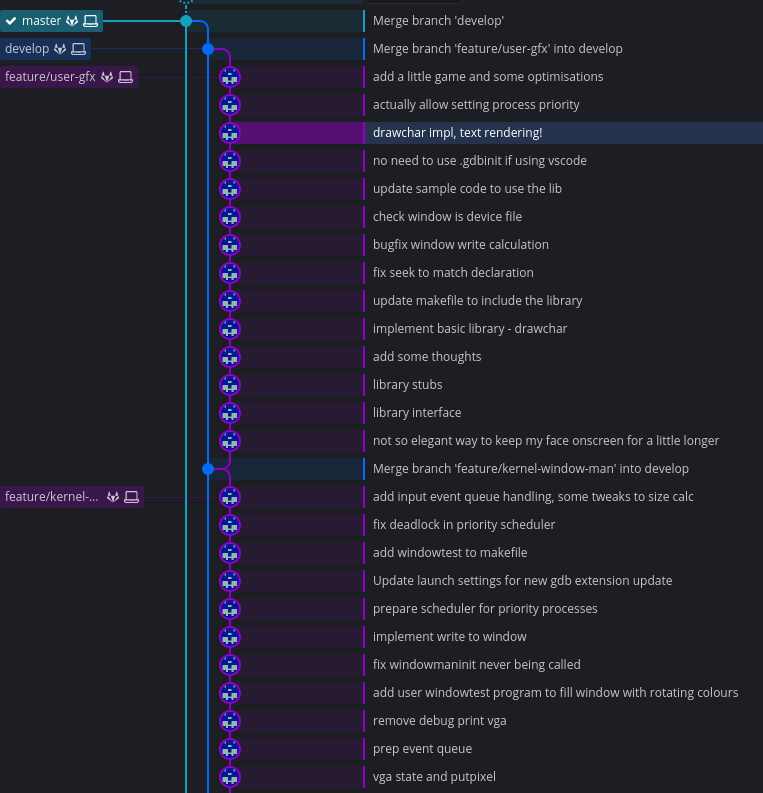
\includegraphics[width=12cm]{Screenshot from 2022-04-27 12-47-49.png}
    \caption{Git commit graph}
    \label{figure:commitgraph}
\end{figure}

\chapter{Results}
\label{chapter3}

<Results, evaluation (including user evaluation) {\em etc.} should be described in one or more chapters. See the `Results and Discussion' criterion in the mark scheme for the sorts of material that may be included here.>

\section{A section}
\lipsum[8]

\subsection{A sub-section}
\lipsum[11]

\section{Another section}
\lipsum[12]

\chapter{Discussion}
\label{chapter4}

\section{Conclusions}
\lipsum[13]

\section{Ideas for future work}
\lipsum[14]



% Adds references to the table of contents.
\addcontentsline{toc}{chapter}{References}

% All your bibtex entries should go in the file called "refs.bib".
\printbibliography
% \bibliography{refs}

% All appendices you have go in a file called "appendices.tex".
\begin{appendices}

%
% The first appendix must be "Self-appraisal".
%
\chapter{Self-appraisal}

\section{Critical self-evaluation}
The development of this project was done well, with all the intended objectives reached
(and arguably, more than just the expected outcomes). The code was written in a structured manner
and well documented with comments. Proper use of version control was also shown through 
git, and uploaded on the GitLab platform.

There were a few challenges related to time management, and with respect to that
the report writing could have been definitely improved if more time were allocated
to iterating through the drafts. In retrospect, the implementation of the
graphics library could have definitely been improved if the issues with QEMU
floating point instructions were resolved, which wasn't possible partly due to 
less than ideal time management.

\section{Personal reflection and lessons learned}
This project was definitely a very challenging undertaking. Initial project progress
was difficult as documentation for VGA hardware is sparse, especially since it is 
considered legacy technology. QEMU's board and VGA card emulation also has no 
format documentation, which resulted in some hours spent looking through QEMU's
source code to find things such as addresses and PCI device IDs.

After the initial hurdle of initiating communication with the emulated card and
being able to display something on screen, development became easier. This experience
also made me realise the importance of documentation and maintainable software. Luckily
the QEMU software is well written so it wasn't too difficult to find what I needed in its
source code. I had prior experience reading through third party source and technical
documentation, and this project challenged those skills.

Overall however, I am happy with what was achieved and I believe the outcomes were
more than satisfactory in consideration to the initial objectives of this project.
At the start of this project I had no idea of the intricacies of low level communication
with graphics hardware, and I managed to develop a fully working graphics implementation
with a user API from scratch.

\section{Legal, social, ethical and professional issues}


\subsection{Legal issues}
Xv6 is made open source with the MIT License, which states any person may
\begin{quote}
    "..use, copy, \textbf{modify}, merge, publish,
    distribute, sublicense, and/or sell copies of the Software..."
\end{quote}
free of charge, given that the full license text and copyright notice
is provided.

As the software is being modified, to comply with the provided license the
original copyright and license will be included in the modified software.
Additionally, there are no references to the original authors' rights to intellectual
property of Xv6 derivatives, so the project - which are original modifications
made to Xv6 - will belong to the author (myself) and should be fine for submission.
\subsection{Social issues}
As there is no processing or storing of personal data there are no social issues.
\subsection{Ethical issues}
There are no ethical issues associated with the project as I am the sole contributor
and no personal data was collected or stored.
\subsection{Professional issues}
There are no professional issues associated with the project as I am the sole contributor.

%
% Any other appendices you wish to use should come after "Self-appraisal". You can have as many appendices as you like.
%
\chapter{External Material}
\begin{itemize}
    \item Xv6 RISC-V OS
    \item QEMU
    \item GNU Compiler Toolchain for RISC-V
    \item Docker
\end{itemize}



%
% Other appendices can be added here following the same pattern as above.
%

\chapter{Project Code Snippets}
\section{Project development environment}
\label{appendix:c:1}
\begin{listing}[H]
    \begin{minted}{docker}
# Download base image ubuntu 20.04
FROM ubuntu:20.04

# LABEL about the custom image
LABEL maintainer="Raka Gunarto <rakagunarto@gmail.com>"
LABEL version="0.1"
LABEL description="COMP2211 xv6 toolchain"

# Disable Prompt During Packages Installation
ARG DEBIAN_FRONTEND=noninteractive

# Update Ubuntu Software repository
RUN apt update

# Install
RUN apt-get -y install wget git build-essential gdb-multiarch qemu-system-misc gcc-riscv64-linux-gnu binutils-riscv64-linux-gnu
    \end{minted}
    \caption{Dockerfile for the development environment}
\end{listing}
\section{Xv6 memory layout}
\label{appendix:c:2}
\begin{listing}[H]
\begin{minted}{c}
// https://github.com/qemu/qemu/blob/e750c10167fa8ad3fcc98236a474c46e52e7c18c/hw/riscv/virt.c#L59
// in qemu riscv "virt" machine, the address space
// for PCI MMIO (memory mapped IO) addresses are
// 0x40000000 - 0x80000000
//
// realistically we should track the base addresses set for
// pci devices and set them dynamically, but since we're only
// supporting one device it's fine to hardcode the address for now
#define VGA_FRAMEBUFFER_BASE 0x40000000L
#define VGA_FRAMEBUFFER_SIZE 0x1000000L

// https://github.com/qemu/qemu/blob/e750c10167fa8ad3fcc98236a474c46e52e7c18c/hw/riscv/virt.c#L58
// in qemu riscv "virt" machine, the configuration space
// starts at 0x30000000 and is 0x10000000 bytes long
#define PCI_ECAM_BASE 0x30000000L
#define PCI_ECAM_LEN 0x10000000L

// https://github.com/qemu/qemu/blob/e750c10167fa8ad3fcc98236a474c46e52e7c18c/hw/riscv/virt.c#L52
// in qemu riscv "virt" machine, the port I/O
// address space starts at 0x3000000 and is 0x10000 long
#define PCI_PIO_BASE 0x3000000L
#define PCI_PIO_LEN 0x10000L
\end{minted}
\caption{/kernel/memlayout.h:69-90, PCI and VGA memory addresses}
\end{listing}

\section{PCI device discovery}
\label{appendix:c:3}
\begin{listing}[H]
    \begin{minted}{c}
void pciinit(void)
{
  uint16 bus; // bus index
  uint8 dev;  // device index

  //-- look through every device (brute-force scan)
  // there are 256 buses, 32 potential devices per bus
  //
  // this is actually very simplified and uses the legacy
  // access method, only looking at PCI Segment Group 0
  // (out of up to 65536 groups)
  for (bus = 0; bus < 256; ++bus)
    for (dev = 0; dev < 32; ++dev)
    {
      //-- calculate offsets
      // volatile pointer because this address is not RAM
      // it's memory mapped PCI registers which can change
      // at any time
      uint32 header_offset = (bus << 16) | (dev << 11);
      volatile uint32 *header = (volatile uint32 *)(PCI_ECAM_BASE + header_offset);

      //-- switch to handle known PCI devices
      // first 32 bits of the PCI header is the
      // device ID and the vendor ID, combined
      // becomes the PCI ID
      switch (*header)
      {
      case 0x11111234:
        setup_vga_card(header);
        break;
      default:
        if (*header != 0xFFFFFFFF)
          printf("pciinit: unknown PCI device: 0x%x\n", header[0]);
        break;
      }
    }
}
    \end{minted}
    \caption{/kernel/pci.c, PCI device discovery through bruteforce scan (legacy access method)}
\end{listing}

\section{VGA modesetting examples}
\label{appendix:c:4}
\begin{figure}[H]
\begin{tabular}{|c|c|c|c|c|c|c|}
\hline
Register name&port&index&mode 3h&mode 12h&mode 13h&mode X\\
\hline\hline
Mode Control&0x3C0&0x10&0x0C&0x01&0x41&0x41\\
\hline
Overscan Register&0x3C0&0x11&0x00&0x00&0x00&0x00\\
\hline
Color Plane Enable&0x3C0&0x12&0x0F&0x0F&0x0F&0x0F\\
\hline
Horizontal Panning&0x3C0&0x13&0x08&0x00&0x00&0x00\\
\hline
Color Select&0x3C0&0x14&0x00&0x00&0x00&0x00\\
\hline
Miscellaneous Output Register&0x3C2&N/A&0x67&0xE3&0x63&0xE3\\
\hline
Clock Mode Register&0x3C4&0x01&0x00&0x01&0x01&0x01\\
\hline
Character select&0x3C4&0x03&0x00&0x00&0x00&0x00\\
\hline
Memory Mode Register&0x3C4&0x04&0x07&0x02&0x0E&0x06\\
\hline
Mode Register&0x3CE&0x05&0x10&0x00&0x40&0x40\\
\hline
Miscellaneous Register&0x3CE&0x06&0x0E&0x05&0x05&0x05\\
\hline
Horizontal Total&0x3D4&0x00&0x5F&0x5F&0x5F&0x5F\\
\hline
Horizontal Display Enable End&0x3D4&0x01&0x4F&0x4F&0x4F&0x4F\\
\hline
Horizontal Blank Start&0x3D4&0x02&0x50&0x50&0x50&0x50\\
\hline
Horizontal Blank End&0x3D4&0x03&0x82&0x82&0x82&0x82\\
\hline
Horizontal Retrace Start&0x3D4&0x04&0x55&0x54&0x54&0x54\\
\hline
Horizontal Retrace End&0x3D4&0x05&0x81&0x80&0x80&0x80\\
\hline
Vertical Total&0x3D4&0x06&0xBF&0x0B&0xBF&0x0D\\
\hline
Overflow Register&0x3D4&0x07&0x1F&0x3E&0x1F&0x3E\\
\hline
Preset row scan&0x3D4&0x08&0x00&0x00&0x00&0x00\\
\hline
Maximum Scan Line&0x3D4&0x09&0x4F&0x40&0x41&0x41\\
\hline
Vertical Retrace Start&0x3D4&0x10&0x9C&0xEA&0x9C&0xEA\\
\hline
Vertical Retrace End&0x3D4&0x11&0x8E&0x8C&0x8E&0xAC\\
\hline
Vertical Display Enable End&0x3D4&0x12&0x8F&0xDF&0x8F&0xDF\\
\hline
Logical Width&0x3D4&0x13&0x28&0x28&0x28&0x28\\
\hline
Underline Location&0x3D4&0x14&0x1F&0x00&0x40&0x00\\
\hline
Vertical Blank Start&0x3D4&0x15&0x96&0xE7&0x96&0xE7\\
\hline
Vertical Blank End&0x3D4&0x16&0xB9&0x04&0xB9&0x06\\
\hline
Mode Control&0x3D4&0x17&0xA3&0xE3&0xA3&0xE3\\
\hline
\end{tabular}
\subsubsection*{Modes}
\begin{itemize}
    \item[3h] - 80x25 text mode
    \item[12h] - 640x480 planar 16 color mode
    \item[13h] - 320x200 linear 256 color mode
    \item[X] - 320x240 planar 16 color mode
\end{itemize}
\caption{VGA register settings for various modes \cite{osdevvga}}
\end{figure}

\section{Boot image}
\label{appendix:c:5}
\begin{figure}[H]
    \centering
    
\includegraphics[width=8cm]{face.png}
    \caption{Boot image, a picture of the project author (Raka Gunarto) with 8 bit colour}
\end{figure}
\begin{listing}[H]
    \begin{minted}{c}
static const unsigned int BOOTIMG_WIDTH = 91;
static const unsigned int BOOTIMG_HEIGHT = 96;
static const char BOOTIMG[] = {
    ...
        17,18,234,161,161,161,162,162,163,24,24,24,25,25,25,25,
	25,25,25,25,25,25,25,24,24,24,24,24,162,162,162,162,
	162,162,162,162,162,161,235,234,233,17,0,0,0,0,17,17,
	17,17,17,17,17,17,18,18,18,18,18,
	185,186,186,186,186,186,209,0,0,0,0,0,0,0,0,0,
	0,0,0,0,0,0,0,0,0,0,0,0,0,0,0,17,
	18,234,234,162,162,162,162,162,24,24,24,24,25,25,25,25,
	25,25,25,25,25,25,24,24,24,24,24,24,162,162,162,162,
	162,162,162,162,162,162,161,235,234,18,0,0,0,0,17,17,
	17,17,17,17,17,17,17,17,17,17,18,
	186,186,186,186,186,186,17,0,0,0,0,0,0,0,0,0,
	0,0,0,0,0,0,0,0,0,0,0,0,17,17,18,18,
	18,233,161,162,162,162,162,162,24,24,24,25,25,25,25,25,
	25,25,25,25,25,25,24,24,24,24,24,24,162,162,162,162,
	162,162,163,162,162,162,161,235,235,233,17,0,0,0,0,0,
    ...
}
    \end{minted}
    \caption{kernel/bootimg.h, code snippet of how the boot image is stored}
\end{listing}
\begin{listing}[H]
    \begin{minted}{c}
  //-- load the bootimage on screen, offset by CPU
  // find how many images fit in a line on the screen
  static const int xfit = 320 / BOOTIMG_WIDTH;

  // figure out the offset for the image based on the CPU id
  const int xoffset = cpu % xfit;
  const int yoffset = cpu / xfit;

  // copy image to screen framebuffer, taking offset into account
  for (int y = 0; y < BOOTIMG_HEIGHT; y++)
    for (int x = 0; x < BOOTIMG_WIDTH; x++)
      vga_framebuffer[(y * 320) + x + (xoffset * BOOTIMG_WIDTH) + (yoffset * 320 * BOOTIMG_HEIGHT)] = BOOTIMG[y * BOOTIMG_WIDTH + x];
  //--
    \end{minted}
    \caption{kernel/vga.c, displaying the bootimage per CPU}
\end{listing}

\section{Window switching code}
\label{appendix:c:6}
\begin{listing}[H]
  \begin{minted}{c}
// uart input interrupts go here
int windowmanintr(int c)
{
    switch (c)
    {
    case C('T'): // control-t switches windows
        if (active_window == ROWS * COLUMNS)
            active_window = 0;
        else
            active_window++;
        drawborders();
        return 0;
        ...
  \end{minted}
  \caption{kernel/windowman.c, handle control character from UART to cycle windows}
\end{listing}

\begin{listing}[H]
  \begin{minted}{c}
static void
drawborders()
{
    const int width = vga_getwidth();
    const int height = vga_getheight();

    const int activewin_row = active_window / COLUMNS;
    const int activewin_col = active_window % COLUMNS;

    // draw vertical lines
    const int xinterval = width / COLUMNS;
    for (int col = 1; col < COLUMNS; ++col)
        for (int y = 0; y < height; ++y)
            if ((col == activewin_col || col - 1 == activewin_col) && (y / (height / ROWS)) == activewin_row)
                vga_putpixel(xinterval * col, y, 0x28);
            else
                vga_putpixel(xinterval * col, y, 0x0F);

    // draw horizontal lines
    const int yinterval = height / ROWS;
    for (int row = 1; row < ROWS; ++row)
        for (int x = 0; x < width; ++x)
            if ((row == activewin_row || row - 1 == activewin_row) && (x / (width / COLUMNS)) == activewin_col)
                vga_putpixel(x, yinterval * row, 0x28);
            else
                vga_putpixel(x, yinterval * row, 0x0F);
}
  \end{minted}
  \caption{kernel/windowman.c, draw window borders, highlight active window in red}
\end{listing}

\section{Window device file functions}
\label{appendix:c:7}
\begin{minted}[breaklines]{c}
// reads max n events from winow event queue, with window specified by the minor
// number in the device file.
// copies a windowevent struct or array into addr,
int windowmanread(int user_dst, uint64 addr, int n, struct file *f)
{
    if (!f)
        return -1;

    if (f->ip->minor >= (ROWS * COLUMNS)) // invalid window
        return -1;

    // find head of event queue
    for (int headidx = 0; headidx < NEVTS; ++headidx)
    {
        // skip if not head
        if (evt_queue[f->ip->minor][headidx].type != HEAD)
            continue;
        
        // return if queue empty
        if (evt_queue[f->ip->minor][(headidx + 1) % NEVTS].type == TAIL)
            return 0;

        // return all events up to n
        evt_queue[f->ip->minor][headidx].type = EVT_KEY; // set to something else, just not HEAD or TAIL
        int evt_count = 0;
        int current_evtidx = (headidx + 1) % NEVTS;
        uint64 caddr = addr;
        for (;
             evt_count < n && evt_queue[f->ip->minor][current_evtidx].type != TAIL;
             current_evtidx = (current_evtidx + 1) % NEVTS,
             ++evt_count,
             caddr += sizeof(struct windowevent))
        {
            either_copyout(user_dst, caddr, &evt_queue[f->ip->minor][current_evtidx], sizeof(struct windowevent));
            evt_queue[f->ip->minor][current_evtidx].type = HEAD;
        }

        return evt_count;
    }

    return 0;
}
\end{minted}
\captionof{listing}{kernel/windowman.c, window device file read function}
\pagebreak
\begin{minted}[breaklines]{c}
// write to window specified by the minor number in the device file.
// bytes are taken from memory specified at addr, length n,
// written to the window starting from the offset in the file struct.
// TODO: some point in the future maybe support bit blitting?
int windowmanwrite(int user_src, uint64 addr, int n, struct file *f)
{
    if (!f)
        return -1;

    if (f->ip->minor >= (ROWS * COLUMNS)) // invalid window
        return -1;

    // check out of bounds
    const int width = vga_getwidth();
    const int height = vga_getheight();
    if (f->off + n > (width / COLUMNS) * (height / ROWS))
        return -1;

    // get framebuffer for direct access
    volatile uint8 *framebuffer = vga_getframebuffer();

    // calculate starting offsets for window
    const int xoffset = (width / COLUMNS) * (f->ip->minor % COLUMNS);
    const int yoffset = (height / ROWS) * (f->ip->minor / COLUMNS);

    // calculate initial offset in window if f->off isn't 0
    int bytes_left = n;
    int current_x = f->off % (width / COLUMNS);
    int current_y = f->off / (width / COLUMNS);

    while (bytes_left > 0)
    {
        // check bytes left will overflow this row
        if (bytes_left + current_x >= (width / COLUMNS))
        {
            either_copyin(
                framebuffer + (xoffset + current_x) + (yoffset + current_y) * width,
                user_src,
                addr,
                (width / COLUMNS) - current_x);
            bytes_left -= (width / COLUMNS) - current_x;
            current_x = 0;
            current_y++;
            continue;
        }

        // fits in this row
        either_copyin(
            framebuffer + (xoffset + current_x) + (yoffset + current_y) * width,
            user_src,
            addr,
            bytes_left);
        bytes_left = 0;
    }

    drawborders();
    return 0;
}
\end{minted}
\captionof{listing}{kernel/windowman.c, window device file write function}

\section{Process priority system call}
\label{appendix:c:8}
\begin{minted}[breaklines]{diff}
--- a/kernel/syscall.c
+++ b/kernel/syscall.c
@@ -105,6 +105,7 @@ extern uint64 sys_unlink(void);
 extern uint64 sys_wait(void);
 extern uint64 sys_write(void);
 extern uint64 sys_uptime(void);
+extern uint64 sys_setpriority(void);
 
 static uint64 (*syscalls[])(void) = {
 [SYS_fork]    sys_fork,
@@ -128,6 +129,7 @@ static uint64 (*syscalls[])(void) = {
 [SYS_link]    sys_link,
 [SYS_mkdir]   sys_mkdir,
 [SYS_seek]    sys_seek,
+[SYS_setpriority]    sys_setpriority,
 [SYS_close]   sys_close,
 };
 
--- a/kernel/syscall.h
+++ b/kernel/syscall.h
@@ -20,4 +20,5 @@
 #define SYS_link   19
 #define SYS_mkdir  20
 #define SYS_seek  20
-#define SYS_close  21
+#define SYS_setpriority  21
+#define SYS_close  22
--- a/kernel/sysproc.c
+++ b/kernel/sysproc.c
@@ -17,6 +17,18 @@ sys_exit(void)
   return 0;  // not reached
 }
 
+uint64
+sys_setpriority(void)
+{
+  int prio;
+  if (argint(0, &prio) < 0)
+    return -1;
+  if (prio != 0 || prio != 1)
+    return -1;
+  myproc()->priority = prio;
+  return 0;
+}
+
 uint64
 sys_getpid(void)
 {
--- a/user/user.h
+++ b/user/user.h
@@ -24,6 +24,7 @@ int getpid(void);
 char* sbrk(int);
 int sleep(int);
 int uptime(void);
+int setpriority(int);
 
 // ulib.c
 int stat(const char*, struct stat*);
diff --git a/user/usys.pl b/user/usys.pl
index 5c787e34826f633b249b63ab338043ea69d64269..2813e432c4dff7703ad5c7203f4cbebb7bbce0e7 100755
--- a/user/usys.pl
+++ b/user/usys.pl
@@ -37,3 +37,4 @@ entry("getpid");
 entry("sbrk");
\end{minted}
\captionof{listing}{Diff at commit da05fd8d to add the setpriority() system call}

\section{High framerate game program code}
\label{appendix:c:9}
\begin{minted}{c}
const int gunsprite_width = 6;
const int gunsprite_height = 8;
const uint8 gunsprite[] =
{
    0x00, 0x00, 0x0B, 0x0B, 0x00, 0x00,
    0x00, 0x00, 0x0C, 0x0C, 0x00, 0x00,
    0x00, 0x0C, 0x0C, 0x0C, 0x0C, 0x00,
    0x00, 0x0C, 0x0C, 0x0C, 0x0C, 0x00,
    0x00, 0x0C, 0x0C, 0x0C, 0x0C, 0x00,
    0x00, 0x0C, 0x0C, 0x0C, 0x0C, 0x00,
    0x0C, 0x0C, 0x0C, 0x0C, 0x0C, 0x0C,
    0x0C, 0x0C, 0x0C, 0x0C, 0x0C, 0x0C,
};

struct coords {
    uint x;
    uint y;
};

static void fire(int bulletx, int bullety, struct coords *bullets)
{
    for (int i = 0; i < 10; ++i)
        if (bullets[i].x == -1 && bullets[i].y == -1)
        {
            bullets[i].x = bulletx, bullets[i].y = bullety;
            break;
        }
}

static int colliding(struct coords c1, struct coords c2, int combinedrad)
{
    uint rsquared = combinedrad * combinedrad;
    uint dx = c1.x - c2.x;
    uint dy = c1.y - c2.y;
    uint distsquared = dx * dx + dy * dy;
    if (distsquared <= rsquared)
        return 1;
    return 0;
}

int main(int argc, char *argv[])
{
    setpriority(1);

    // open the first available window
    window_handle win = window_create();

    struct windowevent evt;
    struct window_dim dim = window_getdimensions(win);

    int gunx = dim.width / 2;
    int guny = (dim.height / 4) * 3;

    const uint bulletrad = 3;
    struct coords bullets[10];

    const uint enemywh = 5;
    struct coords enemies[10];

    for(int i = 0; i < 10; ++i)
    {
        bullets[i].x = -1;
        bullets[i].y = -1;

        int row = i / 5 + 1;
        enemies[i].x = ((i % 5) + row) * (dim.width / 6);
        enemies[i].y = row * (dim.height / 4);
    }
    
    uint score = 0;
    while (score < 10)
    {
        // clear screen
        window_clearscreen(win);

        // handle inputs
        if (window_pollevent(win, &evt, 1) == 1)
        {
            switch (evt.payload)
            {
            case 'a':
                gunx = gunx > 0 ? gunx - 1 : gunx;
                break;
            case 'd':
                gunx = gunx < dim.width ? gunx + 1 : gunx;
                break;
            case ' ':
                fire(gunx + gunsprite_width, guny - 2, bullets);
                break;
            default:
                break;
            }
        }

        // movement
        for(int i = 0; i < 10; ++i)
        {
            // bullets, delete when top of screen reached
            if (bullets[i].x != -1 && bullets[i].y != -1)
                if (--bullets[i].y <= 0)
                    bullets[i].x = -1, bullets[i].y = -1;


        }

        // collisions
        for(int bullet = 0; bullet < 10; ++bullet)
            if (bullets[bullet].x != -1 && bullets[bullet].y != -1)
                for (int enemy = 0; enemy < 10; ++enemy)
                    if (enemies[enemy].x != -1 && enemies[enemy].y != -1 && colliding(bullets[bullet], enemies[enemy], bulletrad + enemywh / 2))
                    {
                        score++;
                        bullets[bullet].x = -1, bullets[bullet].y = -1;
                        enemies[enemy].x = -1, enemies[enemy].y = -1;
                        break;
                    }

        // draw
        window_drawsprite(win, gunx, guny, gunsprite_width, gunsprite_height, gunsprite);
        for(int i = 0; i < 10; ++i)
        {
            if (bullets[i].x != -1 && bullets[i].y != -1)
                window_drawcircle(win, bullets[i].x - bulletrad, bullets[i].y - bulletrad, bulletrad, 0x0C);
            
            if (enemies[i].x != -1 && enemies[i].y != -1)
                window_drawrect(win, enemies[i].x - enemywh, enemies[i].y - enemywh, enemywh, enemywh, 0x0E);
        }

        window_drawchar(win, 8*0, 0, 'S', 0x09);
        window_drawchar(win, 8*1, 0, 'C', 0x09);
        window_drawchar(win, 8*2, 0, 'O', 0x09);
        window_drawchar(win, 8*3, 0, 'R', 0x09);
        window_drawchar(win, 8*4, 0, 'E', 0x09);
        window_drawchar(win, 8*5, 0, ':', 0x09);
        window_drawchar(win, 8*6, 0, ' ', 0x09);
        window_drawchar(win, 8*7, 0, (char)score + 48, 0x09);
    }
    window_destroy(win);
    exit(0);
}
\end{minted}
\captionof{listing}{user/game.c source code}

\end{appendices}


\end{document}

